\setcounter{step}{0}
%------------------------------------------
% information doc
\subsection{Brownies}
\PrepTime{20}
\CookingTime{40}
\CookingTempe{175}
\TypeCooking{Pečenie}
\NbPerson{4}
\Image{0 0 430 430}{images/florentin} %style 2
%------------------------------------------

\begin{ingredient}
%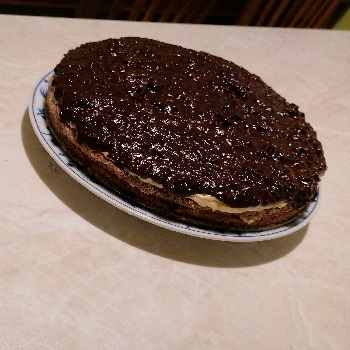
\includegraphics[height=5.5cm]{images/daim}
\def\portions{4}%
\textbf{{\normalsize Ingrediencie (\portions porcie):}}

\begin{main}
	\item 250g horká čokoláda
	\item 250g maslo
	\item 85g orechy
	\item 100g mliečna čokoláda na kúsky
	\item 100g biela čokoláda
	\item 175g hladká múka
	\item 1ČL prášok do pečiva
	\item 4 vajíčka
	\item 1 vanilkový cukor
	\item 300g kryštálový cukor
\end{main}
\end{ingredient}
\begin{recipe}
\textbf{{\normalsize Príprava:}}
\begin{enumerate}

\item{Čokoládu a maslo rozpustíme vo vodnom kúpeli}
\item{Pridáme múku a prášok do pečiva}
\item{Pridáme cukor, vajíčka, vanilkový cukor, orechy, pokrájanú čokoládu}	
\item{Pečieme 40 minút na 175°}

\end{enumerate}
\end{recipe}

\begin{notes}

\end{notes}
\clearpage	